\chapter{\scribe: Transparent Deterministic Record-Replay}
\label{ch:scribe}

\section{Introduction}

Deterministic application record and replay is the ability to record
application execution and deterministically replay it at a later time.
Record-replay has many potential uses, including diagnosing
and debugging applications by capturing and reproducing hard to find
bugs, dynamic application analysis by performing costly
instrumentation on replicas that replay application behavior recorded
on production systems, intrusion analysis by capturing intrusions involving
nondeterministic effects, and fault-tolerance by providing
replicas that replay execution and at the occurrence of a fault, go
live in place of the previously running application instance.  

Many approaches have tried to provide record-replay functionality, but
have suffered from fundamental limitations that make them 
unusable in many cases.  First, most approaches only
support replaying the recorded application execution, and do not allow
the replayed instance to go live and continue normal execution.  This
only works for simple debugging uses.  It does not work for most
scenarios, including any form of debugging that requires the 
replayed instance to go live, such as debugging past the end of a
recorded execution, fault-tolerance which requires the replayed
instance to be able to go live when the primary fails.

Second, previous approaches either require application changes or rely
on specialized hardware that is not always available.  Approaches requiring
application changes impose a recurring development cost on each
application to provide record-replay, and do not work for unmodified
applications.  Approaches requiring specialized hardware rely on
either hardware architectures that exist in simulation only, or assume
the availability of certain performance counters to track
the precise timing of asynchronous events. Such performance counters may not be
available on all hardware platform (e.g. ARM).

Third, previous application transparent approaches either do not
support multiprocessor systems at all, or require using a virtual
machine monitor (VMM) and suffer significant
performance overhead on multiprocessor systems.   This overhead is
imposed on the recording of execution and can result in more than an
order of magnitude reduction in application
performance~\cite{smp-revirt}. Such
overhead is unacceptable even for debugging or analysis. Because
the recording must often be done on a production system to capture and 
identify real bugs for debugging or real application behavior for
analysis, minimizing recording overhead is
crucial to avoid any adverse impact on production application
execution. 

To address these problems, we introduce \scribe{}, the first system
to provide transparent, low-overhead application record-replay and the
ability to go live from replayed execution.  \scribe{}
uniquely combines transparency and low-overhead for application
execution recording based on two principles.  First, \scribe{}
primarily operates at the well-defined interface between applications
and the operating system to record and replay the execution of
multiple processes and threads in a consistent and coordinated manner.
Using a standard interface that applications already use avoids the
need to modify applications to enable record-replay, providing
transparency.  Using a higher-level interface avoids the need to track
and record low-level hardware and operating system
nondeterministic effects that have no impact on enabling deterministic
application replay, reducing overhead. Unlike VMM approaches, it also
enables finer granularity per application record-replay as opposed to
limiting record-replay to an entire operating system instance.
Second, \scribe{} observes that real applications
do frequent system activities such as I/O.  These activities can be
recorded efficiently with relative ease because their timing is
synchronous with the execution of the process performing the
activities.  Using these activities, \scribe{} converts
nondeterministic asynchronous interactions that are difficult to
record and replay efficiently without additional hardware support into 
synchronous interactions that can be recorded in software with low
overhead.  In other words, the timing of an application execution may
be perturbed in a manner that makes it easier to record efficiently
without sacrificing correctness or performance.  

Using these principles, \scribe{} introduces two novel mechanisms to
address the key challenge of 
handling nondeterministic execution.
First, \scribe{} introduces {\em rendezvous points} to record all
nondeterministic interactions between applications and the operating
system that involve system calls.  To be able to go live at any point
during replay, the effect of system calls inside the kernel must be
replayed; replaying just the outcome of system calls in user space is
not sufficient.  \scribe{} does not aim to replay
the exact scheduling order as in the original execution, but instead
uses rendezvous points to make a partial ordering of execution
based on system call dependencies sufficient for deterministic replay.  Since an
exact execution ordering is not needed, \scribe{} does not incur the
associated recording overhead and does not need hardware counters used
to maintain such an ordering.  \scribe{} also logs input data
delivered through system calls to account for nondeterminism due to
external input. 

Second, \scribe{} introduces {\em sync points} that correspond to
synchronous system events such as system calls and certain page faults 
to deterministically record the timing of nondeterministic events like
signals and shared memory interleavings.  For a target process or
thread, an asynchronous event such as a signal or shared memory access
by other processes or threads may occur at any time during the target
process's execution.  This is hard to replay since the event
must be replayed at the exact same instruction in the target process 
as during recording.  \scribe{} defers asynchronous events until sync
points occur to make their timing deterministic so that they are 
easier to efficiently record and replay.  Sync points do not require
hardware counters or application modifications that are necessary with
previous approaches, and do not adversely impact application
performance because they occur frequently enough in real server and
desktop applications due to operating system activities.   

\scribe{} fully supports record and replay of real multi-process
and multi-threaded applications, and  
enables an application to switch from being replayed to
running live at any point in time.
\scribe{} accomplishes all of this in an application transparent
manner, does not require changing, relinking, or recompiling
applications, libraries, or operating system kernels, does not require
any specialized hardware support, does not require a VMM or incur its
associated costs, and works on commodity multi-core and multiprocessor
hardware and operating systems.

We have implemented a \scribe{} Linux prototype and evaluated its
performance on multi-core and multiprocessor systems on a wide
range of real applications.  Our results show for the first time that
(1) sync points are an effective, lightweight mechanism for handling
nondeterminism due to signals and shared memory, (2) sync points occur
often enough in real server and desktop applications that the vast
majority of asynchronous events are handled instantaneously, and even
when events are deferred, they are delayed for 25 to 220\us{} on
average, (3) an operating system mechanism can record-replay real
multi-threaded and multi-process applications, (4) transparent,
low-overhead record-replay
can be done for workloads across a wide range of server and
desktop applications, including Apache, MySQL, Firefox, Acrobat,
OpenOffice, parallel make, and MPlayer.  On a 4-CPU multiprocessor,
\scribe{}'s recording overhead was under 2.5\% for server
applications, and less than 15\% for desktop applications.  These
results show for the first time a new level of transparent record and
replay performance on commodity multiprocessor systems that was not
previously possible. 

This chapter is organized as follows.
\S\ref{scribe:sec:arch} presents an overview of \scribe's architecture.
\S\ref{scribe:sec:syscalls} describes how system calls are recorded and replayed
\S\ref{scribe:sec:memory} describes how shared memory interleavings are recorded replayed.
\S\ref{scribe:sec:rendezvous} covers the {\em rendezvous} event used for ordering access to shared resources.
\S\ref{scribe:sec:sync} describes signal delivery and the recording of asynchronous events.
\S\ref{scribe:sec:results} presents experimental results.
\S\ref{scribe:sec:related} discusses related work.
Finally, \S\ref{scribe:sec:conclusion} presents a summary and concluding remarks of this chapter.

\section{Architecture Overview}
\label{scribe:sec:arch}

\scribe{} can record and replay the execution of a group of processes
and threads from any point in time.  We refer to a group of processes
and threads being recorded or replayed as a {\em session}.  \scribe{}
checkpoints the session at a desired starting time and records the
execution going forward.  It can then restart and replay the
session from the checkpoint.  Checkpoints can be taken at any time,
replay can be done at any later time as well as on another
machine, and replayed execution can go live at any time and continue
normal execution.  \scribe{}'s checkpoint-restart mechanism
provides a consistent checkpoint of process and filesystem state
based on Zap~\cite{dejaview,zap07,zap02}.
We only consider
execution replay on a machine with the same CPU type and features,
such as x86 MMX/SSE instructions, as where the execution was recorded.
For example, a process that uses MMX instructions when it is
recorded cannot be replayed on a machine without MMX instructions.   
We will use Linux semantics to describe how
record-replay is accomplished in further detail.

\scribe{} can start recording execution from a checkpoint of a
session, or it may begin with an empty session by launching a new
process.  To begin recording, a dedicated monitor process attaches
itself to the target process(es), setting a special {\em recording}
flag for each process to indicate that it is being recorded.  This flag is 
inherited via the \code{fork} and \code{clone} system calls, so that
new threads and children of a recorded process will automatically
become part of the recorded session.  Recording takes place in the
context of the recorded process.  \scribe{} uses
stubs to interpose on key operating system kernel entry points to
perform some processing before and after the entry points as needed.
For instance, when a recorded process executes a 
system call, \scribe{} produces events that describe the system
call and its outcome by recording information about the system call
before and after the system call executes.
\scribe{} records by intercepting all
interactions of processes with their environment, capturing
all nondeterminism in {\em events} that are stored in {\em log queues}
inside the kernel.  \scribe{} allocates a private kernel log queue for
each process.  Processes generate events during recording, and
append them to the log queue.  As processes fill their log queues
with events, the monitor pulls them from the queues and
saves them to permanent storage. Recording of a process ends when
the process exits, or when \scribe{} explicitly tells the monitor to
stop the recording.  

\begin{table}[]
\small
\centering
\begin{tabular}{cll}
  \toprule
  {\bf Event}             & {\bf Description}                & {\bf Payload}                                                 \\ \midrule
  {\em hw\_inst}          & hardware instruction trap        & op-code and data, e.g. \code{RDTSC} and counter value  \\
  {\em syscall\_ret}      & system call return               & system call return value                                      \\
  {\em copy\_data}        & data transfer to/from user space & size and contents of data transfer                            \\
  {\em page\_public}      & make page public (not owned)     & page address                                                  \\
  {\em page\_share\_read} & make page shared read-only       & page address, page sequence number                            \\
  {\em page\_own\_write}  & make page owned read/write       & page address, page sequence number                            \\
  {\em rendezvous}        & resource synchronization         & resource sequence number                                      \\
  {\em signal\_receive}   & process received signal          & signal number and info, whether or not in system call     \\
  {\em async\_reset}      & force a sync point               & process user space signature at forced sync point             \\
  \bottomrule
\end{tabular}
\caption{{\bf \scribe Record-Replay Events.}}
\label{scribe:tab:events}
\end{table}

\scribe{} can start replaying a session from the beginning of its
execution or from a restarted session.  To replay, the
monitor launches a new process, or restarts the desired session from
the respective checkpoint and marks all processes with a special
{\em replaying} flag.  A log queue is allocated for each process.
Thereafter, the monitor reads the recorded events from
storage and places the data in the respective log queues. 
 
The recorded events are consumed from the log queues to steer the
processes to follow the same execution paths they had
during recording.  Replay takes place in the context of the
process being replayed.  \scribe{} uses the same stubs for replay as
it did for recording to take control over process execution by
interposing on key operating system kernel entry points.  For example,
when a system call is invoked at replay, \scribe{} consumes an event
from the log queue to determine how to correctly replay the effect of
the system call.  Replay of a process ends when the process
terminates, or when all the recorded events have been consumed.

\scribe{} can also let the session {\em go live}, transitioning it
from controlled replay to live execution, by detaching the monitor
from the processes and flushing all remaining events.  To do this,
\scribe{} must do two things to ensure that the replayed session
is always in a state that allows it to transition to live execution.
First, \scribe{} needs to not only replay the application state in
user space, but also the corresponding state that is internally
maintained by the operating system on the application's behalf.
Second, \scribe{} must ensure that the replayed processes perceive the
underlying system to be the same as at the time of recording.  
System identifiers such as process IDs and network port numbers must
be perceived by processes to remain the same for them to run correctly
after they transition to live execution.  To guarantee this
even if the underlying system has changed, \scribe{} uses operating
system virtualization~\cite{zap02} to encapsulate processes in a
virtual execution environment that provides the same private,
virtualized view of the system when the session is replayed or goes
live as when it was recorded.  Processes only see virtual identifiers
that always stay the same.  Virtual identifiers are transparently
remapped by the environment to real operating system resource
identifiers, and the mappings are updated so that the session can go
live at any time.

The events that \scribe{} records and replays each contains two fields:
the event type, and a payload whose size and contents depend
on the event in question.  Events are not timestamped
because \scribe{} does not replay based on explicit event timing
information, and does not aim to repeat the exact scheduling
order as in the original execution; rather, it ensures that events are
ordered correctly by tracking dependencies among events.  Two events
are {\em related} if they access the same resource and at least one of
them modifies it, for instance a \code{write} and \code{read} on a
pipe.  \scribe{} tracks dependencies to preserve the partial order of
related events during replay.  

Table~\ref{scribe:tab:events} lists all
event types recorded and replayed by \scribe{}.  These events
correctly account for all sources of nondeterministic execution that
are needed to support deterministic replay: nondeterministic machine
instructions, system calls, signals, and shared memory interleavings.
External input is also a source of nondeterminism, but this occurs
through system calls.

The {\em hw\_inst} event is used for nondeterministic machine
instructions which interact directly with the hardware and bypass the
operating system.  There are three such instructions on x86 CPUs.
They all involve reading CPU counters and can be recorded by simply
trapping when they occur.  While trapping is expensive, these
instructions typically occur infrequently; standard binary
instrumentation techniques can be used to optimize performance. 
When a nondeterministic machine instruction occurs, \scribe{} records
a {\em hw\_inst} event whose payload is the instruction type and
its result.  For example, when the \code{RDTSC} instruction occurs,
\scribe{} records a {\em hw\_inst} event whose payload is the
\code{RDTSC} instruction opcode and the 64-bit value of the timestamp
counter.  During replay, \scribe{} returns the recorded result
instead of executing the instruction.

\section{System Calls}
\label{scribe:sec:syscalls}

System calls are the predominant form for processes to interact with
the environment and with other processes. System call interposition is
used to record and replay the execution of system calls.
Unlike other approaches~\cite{liblog,jockey,srinivasan:flashback}, \scribe{} does
not simply feed processes with logged data to simulate the effect of
system calls.  This is not sufficient to enable replayed execution to
go live.  Instead, \scribe{} re-executes system calls during replay to
ensure that the corresponding in-kernel state of a replayed session is
updated properly so that it can transition to live execution at any
time.  We first describe the basics of how \scribe{} handles system
calls, then describe in \S\ref{scribe:sec:rendezvous} how \scribe{}
handles nondeterminism due to system calls that access shared
resources. 

  

\subsection{Record}

During recording, \scribe{} always allows each system call to execute
and records its return value using the {\em syscall\_ret} event so
that the same values can be returned on replay.  The system call
number is not recorded since it will be available on replay when the
process executes the same system call.  
For system calls that create and terminate processes and threads,
namely \code{fork}, \code{clone}, and \code{exit}, \scribe{} also sets
up the log queues, arranges to control the execution of new processes
and threads when they are created, and performs proper cleanup as
processes and threads exit.
For system calls that transfer nondeterministic or external data from
kernel to user space, \scribe{} records the data to the log
queue of the calling process using the {\em copy\_data} event
so that the same data can be output by the system call on replay.
For example, Figure~\ref{scribe:fig:recplay} shows the recording of
\code{gettimeofday}, which outputs to a data structure a time value
which must be recorded. Similarly, all external input data, including
network inputs and data from special devices such
as \code{/dev/urandom}, are delivered via system calls, mainly
the \code{read} system call, and must be recorded.

Data from user space used as input for system calls never
needs to be recorded; it is always deterministic on replay since it
resides in the address space of a replayed process. The only exception
is if a buffer corresponds to mapped I/O memory, whose
contents are logged as well using the {\em copy\_data}
event. Similarly, \scribe{} does not record input from file
descriptors that refer to a local filesystem or to objects such as
pipes, because their state and contents during replay are controlled
by the replay and therefore deterministic.  In contrast, approaches
that use system call simulation must explicitly log such data,
significantly inflating the resulting log size. 

\subsection{Replay}

During replay, \scribe{} replays the system calls of each process
independently, unless system calls access shared resources as discussed
in \S\ref{scribe:sec:rendezvous}.  When a replayed process invokes a
system call, \scribe{} intercepts it and uses the return value from the
corresponding {\em syscall\_ret} event in the log queue of the calling
process as the return value of the system call.  It does not return
the value from executing the actual system call, which may differ and
result in the replay diverging from the recorded execution. 

For system calls that transfer nondeterministic data from kernel to
user space, the data logged in the corresponding {\em copy\_data}
event is also returned on replay.  For example,
Figure~\ref{scribe:fig:recplay} shows the replay of the \code{gettimeofday} 
system call from an event log.

\begin{figure}[t]
  \centering
  \begin{tabular}{lll}

    \toprule

    {\bf Record (action) \hfill $\rightarrow$ }
      & {\bf Event log \hfill $\rightarrow$ }
        & {\bf Replay (action)}
            \\

    \midrule

    ret = gettimeofday(K, NULL)
      &
        & (do nothing)
            \\

    (system call returned)
      & {\em syscall\_ret(ret)}
        &
            \\

    copy out: K$\rightarrow$u (size)
      & {\em copy\_data(size, K)}
        & copy out: K$\rightarrow$u (size)
            \\

    return(ret)
      &
        & return(ret)
            \\
    \bottomrule
  \end{tabular}

  \caption{{\bf Record-Replay of \code{gettimeofday}.}
    { 
      To record, \scribe{} invokes the system call with an in-kernel
      buffer (K), logs the return value and input data, copies the
      data to the user buffer (u) and returns. To replay it copies
      the logged data to the user space buffer and returns the logged
      return value.
    }
  }
  \label{scribe:fig:recplay}
\end{figure}

Beyond dealing with the return value and nondeterministic data, we can
classify system calls into two categories: idempotent and non-idempotent.
Idempotent system calls do not modify the internal kernel state, and
therefore the underlying call does not even need to be executed. These
system calls typically query resource identifiers, such
as \code{getpid}, \code{getppid}, \code{getuid} and \code{getgid}, or 
transfer data about resources, such as \code{uname}, \code{getrusage}, 
\code{time}, \code{getitimer}, \code{gettimeofday},
and \code{sysinfo}.  Non-idempotent system calls modify system state
and therefore replay typically requires executing the underlying
system call. 

The processing of non-idempotent system calls varies for 
different system calls.  Most of these system calls are replayed
directly by executing them. Examples include \code{setsid},
\code{brk}, reading from and writing to a pipe, etc.  By executing
these system calls, \scribe{} guarantees that the state of all the
resources that belong to the session is correct at all times, and the
session may safely stop replaying, go live, and proceed to execute
normally. If a system call execution that was successful in the
original application execution fails during replay, \scribe{} aborts
the replay. 

  

For system calls that create and terminate processes and threads,
namely \code{fork}, \code{clone} and \code{exit}, \scribe{} sets up
the log queues, arranges to control the execution of new processes
and threads when they are created, and performs proper cleanup as
processes and threads exit. When creating processes and threads during
replay, \scribe{} relies on the underlying virtual namespace
to provide a method to select predetermined virtual process
identifiers so that processes can reclaim the same set of virtual
resource identifiers they had used during recording.  The same is true
for other system calls that allocate resources with identifiers
assigned by the kernel, such as IPC identifiers.

For system calls that carry out external I/O, the internal state of
file descriptors, such as file position, is updated even though data
may not be explicitly sent or received through the file descriptors. 
For example, for external input, \scribe{} replays the data to the
application from the log rather than fully execute the 
system call.  

For system calls that accept wildstar (catch-all) arguments,
such as \code{mmap} and \code{wait}, \scribe{} already knows the
outcome of the system call, e.g., which address or process was
selected. For deterministic replay, it simply substitutes
that outcome for the wildstar argument.

    

\subsection{Go Live}
\label{scribe:sec:golive}

In most cases, executing recorded system calls during replay is
sufficient to automatically replay the kernel state correctly, due to
the deterministic behavior of the application and the operating
system. For example, when an application creates and then writes to a
pipe, the kernel internally allocates a pipe object, populates the
process's file table with suitable file descriptors, and then places
data in the pipe's internal buffer. During replay, the application
will issue the same system calls, in the same partial order, and the
kernel will deterministically behave in the same way and reconstruct
the same internal state.

However, internal kernel state that is related to external entities is
unique in that it interacts with, and is affected by, state that is
not controlled by the session. How such state is handled is predicated
on what is assumed about the external environment when a session goes
live. We identify two scenarios: {\em stand-alone} execution assumes
that the original external links are non-existent, e.g. in debugging
use case, and {\em switch-over} execution assumes that they remain 
as is, e.g. for replica execution.

In stand-alone replay, internal kernel state linked to outside the
session would become meaningless once the session goes live. Thus,
\scribe{} needs to cast meaningful state that gracefully reflects the
new status of the resources it represents. It does so by partially
executing select system calls that create or manipulate this state.

To illustrate this concept, consider network connections created via
\code{connect} and \code{accept} system calls. Since \code{connect}
attempts to create a connection to the external world, \scribe{} skips
its invocation during stand-alone replay. A successful \code{accept}
will receive an incoming connection into a new socket. To replay
this, \scribe{} creates a new, disconnected, socket instead. The end
result in both cases, is that the socket remains closed; should the
application thereafter go live, it will perceive a network disconnect
upon the next attempt to read or write the socket.
  
  

Switch-over replay, on the other hand, introduces two additional
complexities. First, it requires that the transition to live execution
occur transparently, in a way that external entities, such as remote
connections, would not notice. Second, replaying of kernel state is
no longer deterministic, since it is affected by the interaction with
external entities, e.g. the random choice of sequence numbers for TCP
connections, and interleaved order of incoming messages.

\scribe{}'s approach is to maintain a compatible, but not necessarily
identical, internal kernel state during replay. This avoids
numerous intricacies involved in identifying, recording and replaying
nondeterministic events of, for instance, the network stack. A key
observation is that the replay does not interact with the real world
until it goes live. It is permissible to have differences
in the internal state, provided that when the transition to live
execution takes place, the state is consistent with what was previously
published to, and hence expected by, the external world.

Consider, for instance, internal kernel state that corresponds to
network communication. For protocols that lack reliability guarantees,
such as UDP, \scribe{} need only maintain the corresponding network
endpoint, and may safely ignore buffered or
in-transit data. For connection-oriented protocols, like TCP, it
records important events that permanently affect the internal
state. This includes selection of port number, updates of sequence
numbers and timestamps, setup of timer expirations, and acknowledged
received data. Unacknowledged received data is not tracked since it
will be retransmitted. Data in the send buffers is not logged either
because it will be deterministically reproduced by replaying the
application.

  
\section{Shared Memory}
\label{scribe:sec:memory}

Replaying shared memory interleaving is critical for deterministic
replay, especially on multiprocessor machines.  Memory sharing happens
either explicitly when multiple processes share a common shared
mapping, or implicitly when the entire address space is shared,
e.g. with threads.  The main tool to monitor and control memory
access in software is the page protection mechanism.  Replaying the
order of memory accesses efficiently in software is fundamentally
difficult since one process may access shared memory asynchronously
with, and at any arbitrary location within, another process's
execution.

   

\scribe{} addresses this problem by introducing page ownership
management. Because of spatial and temporal locality, a process
typically accesses multiple locations on a page during a given time
interval.  If we can guarantee that no other processes modify that
page during the same time interval, then the page can be treated like
private memory for that process during that interval.  There would be
no need to track memory accesses since there are no nondeterministic
shared memory interleavings. This scheme requires a
protocol to manage page ownership transitions, and a method to ensure
that such transitions occur at precisely the same location in the
execution during both record and replay. The latter problem is the
key challenge, and is discussed in \S\ref{scribe:sec:sync}.

\scribe{} employs a concurrent read, exclusive write (CREW)
protocol~\cite{crew,instant-replay} for shared memory access, but with
additional optimizations.  A state
field of a page indicates whether it is un-owned ({\em public}), owned
exclusively for read and write ({\em owned\_write}) or shared for read
by one or more processes ({\em shared\_read}). A process that owns
a page exclusively has its PTE set as read and write. A process that
shares a page has the PTE set to read-only. Otherwise the respective
PTE will remain invalid to prevent access. A page that is shared for
reading continuously tracks its list of readers, and an exclusively
owned page tracks its writer (owner).

\begin{figure}[t]
  \small
  \centering
  \begin{tabular}{lll|l}

    \toprule

    {\bf Record (action) \hfill $\rightarrow$ }
      & {\bf Event log \hfill $\rightarrow$ }
        & {\bf Replay (action)}
          & {\bf User-space}
            \\

    \midrule	

    copy in: u$\rightarrow$K (size)
      &
        & copy in: u$\rightarrow$K (size)
          & {\em (A) write(fd, u, size)}
            \\

    rendezvous(A, fd.inode)
      & {\em (A) rendezvous(SEQ)}
        & rendezvous(A, fd.inode)
          &
            \\

    ret = write(fd, K, size)
      &
        & ret = write(fd, K, size)
          &
            \\

    (system call returned)
      & {\em (A) syscall\_ret(ret)}
        & (system call returned)
          &
            \\

    return(ret)
      &
        & return(ret)
          &
            \\

    \multicolumn{1}{c}{ $\cdots$}
      & \multicolumn{1}{c}{ $\cdots$}
        & \multicolumn{1}{c}{ $\cdots$}
          & \multicolumn{1}{|c}{ $\cdots$}
            \\

    rendezvous(B, fd.inode)
      & {\em (B) rendezvous(SEQ+1)}
        & rendezvous(B, fd.inode)
          & {\em (B) read(fd, u, size)}
            \\

    ret = read(fd, K, size)
      &
        & ret = read(fd, K, size)
          &
            \\

    return ret
      & {\em (B) syscall\_ret(ret)}
        & return ret
          &
            \\

    copy out: K$\rightarrow$u (size)
      &
        & copy out: K$\rightarrow$u (size)
          &
            \\

    return(ret)
      &
        & return(ret)
          &
            \\

    \bottomrule	

  \end{tabular}

  \caption{{\bf Rendezvous Points.}
    {
      Process $A$ must pass a rendezvous point before it can invoke
      the system call in both record and replay. Process $B$ must do
      so too, but with a larger sequence number, thus preserving their
      relative order. The data itself is deterministic and not logged.
    }
  }
  \label{scribe:fig:rendezvous}
\end{figure}

Transitions between the page states are as follows. A {\em public} page
becomes {\em shared\_read} or {\em owned\_write} on the first read or
write access, respectively. An {\em owned\_write} page becomes {\em
shared\_read} when another process attempts to read from it; the owner
process will give up exclusive access and downgrade its PTE to be
read-only. An {\em owned\_write} page can also change owner, in which
case the old owner will give it up and invalidate its own PTE, while
the new owner will adjust its PTE accordingly. A {\em shared\_read}
page becomes {\em owned\_write} when the page is accessed for writing.
Finally, a page becomes {\em public} when all processes that have a
right to access terminate.  

Transitions between page states occur as a result of page faults,
which indicate that the faulting process is requesting access to a
given page.  \scribe{} employs two optimizations to reduce the
occurrence of these faults.  First, \scribe{} optimizes for the
common memory access pattern of reading then writing the same, or
nearby, memory addresses.  For this pattern, the standard CREW protocol
incurs two page faults: a read fault makes the page {\em shared\_read}
and a write fault makes it {\em owned\_write}. To avoid this cost,
\scribe{} marks pages when they experience a double fault by the same
process. A marked page will transition directly to {\em owned\_write}
on subsequent page faults, whether they are reads or writes. Finally,
\scribe{} clears the flag if the number of page faults exceeds a defined
threshold, to adjust its behavior for possibly changing memory access
patterns.  

Second, \scribe{} optimizes to reduce frequent transfers of page
ownership.  This can occur among multiple threads due to true or
false data sharing.  Such page ping-ponging can cause 
thrashing, especially when multiple pages are involved.  For instance,
a thread that uses two pages repeatedly in a tight loop may
lose ownership of one page while faulting on the other. To
mitigate this, \scribe{} defines a minimal ownership retention
interval that begins with an ownership change.  Ownership transitions
are disallowed until the interval expires.
The length
of the interval is comparable to a standard scheduler time quantum so
that a running process is likely to
complete its scheduled
time quantum of work.

  

\scribe{}'s page ownership management mechanism requires updating
PTEs.  To support threads without high
overhead due to TLB invalidations, we use private page tables to
track thread shared memory accesses.  All threads associated with
a process share a common
page table for reference, but each thread uses its own private
page table.  The reference page table maintains the current
state of all pages.  When a thread causes a page fault, \scribe{}
consults the corresponding entry in the reference page table and
copies the PTE to the thread's private table. This is inexpensive
because it only flushes a single TLB entry on the local CPU, instead
of a costly inter-processor interrupt followed by a global TLB flush.
The reference page table
is explicitly updated when the process's
address space layout is modified, e.g. through \code{mmap}, \code{munmap} and
\code{mprotect}. For a
single thread, the private page table directly mirrors the reference
page table. 

 

	

 

  
\section{Rendezvous Points}
\label{scribe:sec:rendezvous}

System calls that access shared resources may cause nondeterminism
arising from the order of the execution of {\em related} system calls
that access the same resource and at least one of them modifies it.
For instance, a \code{write} and a \code{read} on the same pipe are
related. The order in which related system calls occur needs to be
recorded so they can be deterministically replayed.  It is crucial
to do this in a way that does not degrade performance and scalability
on multiprocessor systems.

By operating at the system call level, \scribe{} introduces a novel
mechanism to address this problem by capturing concurrency at the same
granularity as the operating system.  The only requirement is
to record and replay the order of any two related system calls.
Related system calls occur from accessing shared resources.  We
observe that the operating system kernel must already provide
locations where access to shared kernel objects is serialized for
correctness.  \scribe{} can thus mimic these serialized access
points to record and replay the order of any two related system calls.

\scribe{} introduces {\em rendezvous points}, locations at which
system call ordering is tracked during recording and enforced during
replay.  Because related system calls occur from accessing shared
resources, \scribe{} synchronizes access to each such resource by
converting all locations in which shared resources are accessed into
rendezvous points.  Since these locations are already used by the
kernel to serialize access to an instance of a shared resource,
rendezvous points do not reduce the scalability or concurrency of the
kernel.  Our approach avoids the overhead of maintaining an exact
execution ordering of system calls and makes a partial ordering of
execution based on system call dependencies sufficient for replay.

  

Rendezvous points are recorded by associating each resource instance 
with a wait queue and a unique sequence number counter. At
any time, exactly one process may be executing inside a given
rendezvous point, while others must block until the resource is
released.  During recording, a process that attempts to access a
shared resource will first pass through the corresponding rendezvous
point.  By doing so, it will increment the sequence number and
generate a matching {\em rendezvous} event. The sequence number in the
{\em rendezvous} event indicates the exact access order for the
resource, which can be used to enforce the order during replay.
Figure~\ref{scribe:fig:rendezvous} shows the recording of
the \code{write} and \code{read} system calls using rendezvous points
and the resulting log. 
Ideally, for each rendezvous point, we could reuse the respective
kernel locking primitive already in place for the associated
resource, but this involves kernel changes.  To avoid changing the
underlying kernel, \scribe{} resorts to its own, separate mutex to
interpose transparently at well-defined kernel entry points.
\S\ref{scribe:sec:results} shows that our approach incurs low overhead
on real applications. 

During replay, \scribe{} replays the system calls of each process
independently from other processes until reaching a rendezvous point.
\scribe{} repeats the order in which processes executed through
rendezvous points when originally recorded by only permitting the
process with matching (smallest) sequence number to enter at any
single time. Processes with higher sequence numbers will block and
wait for their turn.  \scribe{} exploits these rendezvous points to
preserve the partial ordering of related system calls during replay.
Figure~\ref{scribe:fig:rendezvous} illustrates the use of rendezvous points
when replaying the \code{write} and \code{read} system calls.

  

Table~\ref{scribe:tab:rendezvous} lists all categories of related systems
calls, and the respective resources used for rendezvous points.
\scribe{} defines a special pseudo rendezvous point that
is used for system calls that access properties global to the
execution environment, such as \code{syslog}, \code{sethostname}, and
\code{settimeofday}. It is also used for system calls that modify
system-wide state such as mount points, pseudo terminals, etc.  This
preserves their order to ensure that the settings are accurate should
the system go live at any point.

  

For system calls that operate on open file objects, including files,
devices, network sockets, and pipes, \scribe{} uses inodes as
rendezvous points.  Inodes are referenced by a variety of file-related
system calls such as \code{read}, \code{write},
\code{close},
and \code{fcntl}.  Since most
file-related operations are re-executed during replay, this ensures
that they occur in the proper order for a given inode.
 
Similarly, for system calls that operate on System V IPC
objects, including message queues, semaphores, and shared memory,
\scribe{} uses the respective System V IPC resources as rendezvous points.

Shared memory pages that are file mapped can be accessed either via
direct memory references, or through the virtual filesystem (VFS)
using \code{read} and \code{write}. By definition, access via
system calls will bypass the page protection mechanism that enforces
the CREW protocol. For example, through the VFS, a process may change a
page that it does not own. To prevent deadlocks and ensure consistency
with CREW, \scribe{} associates rendezvous points with these pages.
This guarantees that the two methods to access shared mapped pages are
properly coordinated, and that their order is preserved between record
and replay.

\begin{table}[]
\centering
\begin{tabular}{ll}
  \toprule
  {\bf System call category}     & {\bf Rendezvous resource} \\ \midrule
  actions on globals             & global (pseudo)           \\
  actions on open file objects   & {\tt inode} of the file   \\
  actions on IPC objects         & IPC objects               \\
  read/write shared mapped files & memory page               \\
  actions on pathnames           & filesystem mount point    \\
  create file descriptors        & file descriptors table    \\
  modify memory layout           & memory descriptor         \\
  actions on process properties  & process descriptor        \\
  \bottomrule
\end{tabular}
\caption{{\bf List of Rendezvous Points Categories.}}
\label{scribe:tab:rendezvous}
\end{table}

For system calls that operate on filesystem pathnames, including
\code{open}, \code{unlink}, \code{creat}, \code{fifo}, \code{access},
\code{stat}, \code{chmod}, \code{chown}, \code{execve}, and
\code{chroot}, \scribe{} must be able to track their ordering to
replay them correctly because they may modify the state of the
filesystem by creating, deleting and modifying attributes of files.
\scribe{} uses filesystem mount points as rendezvous points, but uses
them at the VFS layer, not the system call
layer.  Using them at the system call layer would serialize
all filesystem accesses during recording and cause high overhead.
Instead, we observe that the order in which system calls that act 
on pathnames view and modify the filesystem state depends on
the order of pathname lookup progress at the 
VFS layer.  The VFS performs pathname traversals one component at a
time, always holding the lock of a parent directory while accessing or
modifying its contents.  To reproduce the order of system calls
that act on pathnames, it suffices to record the order of pathname 
traversal.  \scribe{} achieves this by interposing on the VFS pathname
traversal to increment the sequence number for the rendezvous point
associated with the mount point.  Since \scribe{} is only concerned
with actions that affect the existence or access permissions of files,
it only needs to increment the sequence number for system calls
that perform such operations.  This imposes negligible overhead during
recording.  

In the presence of threads, \scribe{} must also use rendezvous points
to track system calls that create file descriptors, modify memory
layout, and modify process properties or credentials, since those
per process resources are shared among threads.  
For system calls that create file descriptors, such as
\code{open}, \code{pipe}, and \code{fifo}, \scribe{} uses the calling
process's file descriptor table as a rendezvous point.  \scribe{}
cannot rely on an underlying inode for synchronization, because it
does not yet exist.  
For system calls that modify the memory layout, such as \code{brk},
\code{mmap}, \code{munmap}, and \code{mprotect}, \scribe{}
uses the calling process's memory descriptor as a rendezvous point.  
For system calls that modify process properties and credentials,
including \code{setuid}, \code{setgid}, \code{setpgid}, \code{setsid},
\code{setrlimit}, \scribe{} uses the process descriptor as the
rendezvous point.  This is convenient because the properties belong to
a process, and the affected operations are performed in that process's
context. 

\scribe{} also uses the process descriptor rendezvous point
to ensure correct ordering among system calls that modify the
filesystem view of a process, such as \code{chroot} and \code{chdir}.
System calls that are re-executed on replay and
implicitly rely on process properties and credentials must also use the
rendezvous point associated with the process descriptor. For example,
\code{open} and \code{access} use a process's user and group
identifiers to decide if it has sufficient permissions to operate on a
file, \code{kill} uses capabilities to permit a signal, and
\code{setpgid} uses a process's session identifier. 

Executing a system call may result in recording multiple
rendezvous events.  The categories of rendezvous points listed in
Table~\ref{scribe:tab:rendezvous} are not mutually exclusive.  For example,
running \code{open} on a file already opened by another process, will
result in a rendezvous event for the global resource, for the process
descriptor, and for the inode resource.  

\section{Sync Points}
\label{scribe:sec:sync}

\begin{figure}[t]
  \small
  \centering
  \begin{tabular}{llll|l}

    \toprule

    & {\bf Record (action) \hfill $\rightarrow$ }
      & {\bf Event log \hfill $\rightarrow$ }
        & {\bf Replay (action)}
          & {\bf User-space}
            \\

    \midrule

    (a)
    & (do nothing)
      & (queue {\em sig} on {\em B})
        & (do nothing)
          & {\em (A) kill(B, sig)}
            \\

    & return(0)
      & {\em (A) syscall\_ret(0)}
        & return(0)
          &
            \\

    & \multicolumn{1}{c}{ $\cdots$}
      & \multicolumn{1}{c}{ $\cdots$}
        & \multicolumn{1}{c}{ $\cdots$}
          & \multicolumn{1}{|c}{ $\cdots$}
            \\

    & kill(B, sig)
      & {\em (B) signal\_received(sig)}
        & kill(B, sig)
          & {\em (B) sync point}
            \\

    \midrule

    (b)
    & (A) (stall)
      & (queue {\em ADDR} on B)
        & (A) (stall)
          & {\em (A) read page ADDR}
            \\

    & \multicolumn{1}{c}{ $\cdots$}
      & \multicolumn{1}{c}{ $\cdots$}
        & \multicolumn{1}{c}{ $\cdots$}
          & \multicolumn{1}{|c}{ $\cdots$}
            \\

    & (B) (adjust PTE)
      & (B) {\em page\_share\_read(ADDR)}
        & (B) (adjust PTE)
          & {\em (B) sync point}
            \\

    & (A) (adjust PTE)
      & (A) {\em page\_share\_read(ADDR)}
        & (A) (adjust PTE)
          & {\em (A) woken up}
            \\

    & (A) read page ADDR
      & 
        & (A) read page ADDR
          &
            \\

    \bottomrule	

  \end{tabular}

  \caption{{\bf Asynchronous Events Record-Replay.}
    { 
      (a) The sender of a signal always skips the call and notifies
      the receiver instead; The receiver handles and logs the signal
      when it reaches a sync point.
      (b) Assume process $B$ owns a page for writing. Process $A$
      faults reading from the page, notifies the owner, and blocks;
      When $B$ reaches a sync point, it downgrades the page state (and
      PTE) to read-only, and logs a memory event; Finally, $A$ updates
      its own PTE and resumes execution.
    }
  }

  \label{scribe:fig:recasync}
\end{figure}

Asynchronous events cause nondeterminism arising from the timing of
their occurrence.  Replaying asynchronous events is challenging
because it requires that a recorded event occur at the exact same
place in the process's instruction stream as during recording. It is
difficult because it could have occurred at an arbitrary location
during the execution. The two predominant examples of asynchronous
events are signal delivery and page ownership transfers for shared
memory, described in \S\ref{scribe:sec:memory}.

Consider signal delivery.  Signals are delivered in two steps.  First,
the sender process sends a signal to the target process, which is
marked as having a signal pending.  Second, the target process detects
the pending signals when it resumes from kernel space, and handles
them.  If the target process is executing in user space, an
inter-processor interrupt will force it into kernel space, where it 
will detect the pending signals.  Replaying this behavior requires
interrupting the target process at the exact same instruction as
during its original execution.  This is difficult because the
interrupt could have occurred at any time during execution.

Consider page ownership transfers for managing shared memory.  As
described in \S\ref{scribe:sec:memory}, a process requesting access to
a shared memory page will page fault if it does not have the necessary
ownership to read or write the page.  This fault occurs asynchronously
with the execution of the process that owns the page.  Replaying this
behavior requires interrupting the owner process at the exact same
instruction at which ownership is transferred to the requesting
process as during its original execution.  This is difficult because
the fault could have occurred at any time during its execution.

Attempting to address this problem while providing application
transparent record-replay, previous
approaches~\cite{bressoud-tft,bressoud,revirt,smp-revirt} 
have relied on hardware providing a cycle accurate instruction
counter~\cite{slye96}.  The respective counter value at which the
asynchronous event occurs is logged so that during replay, the event
can be replayed at the exact same counter value.  The fundamental
problem with this approach is that such counters are not available on
many CPUs, and even when available, often do not have required degree
of accuracy because they were not designed for this purpose.  They
work for performance measurements where occasional missed counts in
various corner cases are not problematic, but do not work for
record-replay where precise instruction counts are required. 

\scribe{} takes a fundamentally different approach to address this
problem by introducing a novel and efficient mechanism that makes
asynchronous events much easier to record and replay by deferring
their delivery until the nearest synchronous system event.  This is
done by introducing {\em sync points} to represent synchronous system
events which are used for this purpose.  Sync points
are locations in a recorded process's execution which (1)~cause the
process to enter kernel space by executing the following instruction,
and (2)~are guaranteed to do so deterministically during replay
(assuming a faithful execution prior to reaching there). Since
\scribe{} interposes on these kernel entry points, it can easily
record the occurrence and location of sync points. Calling a system
call and triggering a trap due to division by zero are two examples of
sync points. Certain page faults, namely due to invalid memory access,
or due to memory sharing also qualify.
However, page faults due to copy-on-write or memory paging do not
satisfy the second requirement.

\subsection{Signal Delivery}
\label{scribe:sec:signaldelivery}

During recording, \scribe{} defers the delivery of an asynchronous
signal until the target process is at a sync point.  This allows
\scribe{} to easily determine the exact instruction at which the signal
is delivered.  If the target process is in user space, \scribe{} queues
the signal
until the process reaches a sync
point, such as a system call, and therefore synchronously enters the
kernel.  This effectively transforms the asynchronous nature of
signals into synchronous behavior.  Specifically, when a process
enters kernel space, it first checks if it has any pending deferred
signals.  If so, \scribe{} will deliver them to the process and log a
corresponding {\em signal\_receive} event for each delivered signal,
then force it to return to user space to handle them.  In the case of a
sync point due to a system call, it will also rewind the instruction
pointer so that the process will re-issue the system call. 
If the target process is in kernel space, it is already at a sync point
and the signal is delivered immediately. 

Note that some signals are synchronous in that they are the direct
result of an action of the process, like \code{SIGSEGV},
\code{SIGFPE}, \code{SIGBUS}.  These occur while the process is in
user space, and cannot be deferred for a later time.  They already
force the process into kernel space and can therefore be delivered and
handled on the spot.  These signals do not need to be logged because
they are deterministic, and will implicitly occur as part of the
replay once the condition occurs that had triggered them in the
original recording.

During replay, the sender process skips the system call that
sends the signal and continues execution. Instead, signal
delivery is deterministically replayed at the occurrence of sync
points in the execution of the receiving process. When
a process enters kernel space as it reaches a sync point, \scribe{}
examines the next event in its log queue; if it finds a
{\em signal\_receive} event, it will
deliver the designated signal to the process. The process will
handle the signal as soon as it resumes to user space.
Figure~\ref{scribe:fig:recasync}a illustrates record-replay of signals.

One set of signals, \code{SIGSTOP} and \code{SIGCONT}, are treated
differently.  Unlike other signals, which are replayed by arranging
for the process to receive the desired signal, \scribe{} does not
resend \code{SIGSTOP} as it would interfere with the replay. Because
replay is performed in the context of the process, a stopped process
will never check its queue for the corresponding
\code{SIGCONT} signal. Instead \scribe{} maintains the process in a
``stalled'' state in kernel space, and examines the following events in
the queue. The next event may be either another {\em signal\_receive}
event or a page ownership transition event, as discussed in
\S\ref{scribe:sec:memory}. \scribe{} 
processes the remaining events in the queue
until it encounters a \code{SIGCONT}, and then allows the process to
resume execution.  When a session that contains a stalled process
prepares to go live, \scribe{} arranges to send the previously
skipped \code{SIGSTOP} to the process, forcing the process into the
proper kernel state.

  

\subsection{Page Ownership Transfer}
\label{scribe:sec:pageownership}

Page state transitions are allowed to only take place when \scribe{}
can conveniently track, and later replay them. We draw the following
analogy to signal delivery: the process that page faults and the page
owner(s) are analogous to the sender and the receiver of a signal,
respectively.  \scribe{} converts asynchronous memory events into
synchronous ones by deferring them until the owner process reaches a
sync point.

When a process tries to access an owned page it notifies the owner
and, unlike with signals, blocks until access is granted.  Conversely,
owner processes check for pending requests at every sync point and, if
necessary, give up ownership. Figure~\ref{scribe:fig:recasync}b illustrates
record-replay of memory interleaving.  Note that page faults due to
the memory interleaving under the CREW protocol contribute
significantly to the pool of sync points, adding to system calls.

Although transfer of page ownership is always performed by the owner
process(es), there is one exception to this rule due to interaction of
blocking system calls and shared memory.  When an owner of a page
blocks inside a system call, it cannot transfer its page
ownership to another process.  This can cause long delays in
ownership transfer, and
even lead to a deadlock if, for
example, the owner blocks on a read from a pipe, and the other process
stalls on a memory access while attempting to write into the same
pipe.

To address this problem, \scribe{} guarantees that user space
shared memory is not accessed by an owner process when it is executing
a system call.  If another process needs to access a shared memory
page owned by the calling process, \scribe{} can simply transfer
ownership to the requesting process knowing that the original owner
process will not access shared memory because it is executing a system
call.  There are no shared memory interleavings to track between the
original owner process and the requesting process.  \scribe{} can
just identify the location in the original owner's instruction stream
at which this ownership transfer occurs as being the occurrence of the
system call, which it already logs.

More specifically, since various system calls transfer data between
the kernel and user space which could involve a shared page owned by
the calling process, \scribe{} uses an in-kernel staging area where it
temporarily stores both input and output data.  As a result, only the
staging area, not user space memory, is accessed by the calling
process during system calls.  \scribe{} flags an owner that enters a 
system call as a {\em weak-owner} until the system call completes.
This flag indicates that other processes may promptly revoke ownership
of pages that it holds whose retention interval expired. If during the
system call the owner also becomes blocked, \scribe{} flags it as a
{\em sleep-owner} until it resumes execution. This flag indicates that
other processes may promptly revoke ownership of any pages that it
holds.  PTEs of the requesting processes and the owner are updated
promptly to reflect these actions.

\subsection{Signature Record and Replay}

Deferring signals and page ownership transfers may incur a performance
penalty by increasing the latency of signal delivery and page faults
on shared memory, respectively.  \scribe{}'s approach to recording and
replaying asynchronous events is predicated on the assumption that
sync points occur frequently enough in real applications, since they
often enter kernel mode by executing system calls or causing page
faults. Based on this assumption, we expect any performance overhead
to be low in practice.  \S\ref{scribe:sec:results} presents
experimental results that validate our assumption.

In addition, for tracking shared memory, it assumes that real
applications do not typically use user space-only spinlocks or related
mechanisms.  For example, consider a thread that reads from a memory
location in a busy loop until it finds a positive value, and another
thread that intends to write a positive value to that location.
Assume that the former thread becomes the owner of the page.  The
threads are now deadlocked, since the second thread waits for the
first thread to give up the ownership for the page, and the first
thread waits for the second one to change the value in the memory.
This assumption may be incorrect for certain applications.

Although the likelihood of either scenario is not common in real
applications, \scribe{} also provides a novel but more heavyweight
mechanism to record and replay asynchronous events that were
deferred for too long due to an unlikely absence of sync points.
During recording, if a signal, or a page ownership transfer, has been
deferred for a period that exceeds a predefined threshold, \scribe{}
switches to a different mechanism.
\scribe{} sends the target process a reserved signal that forces it
into kernel mode.  By using a reserved signal, we ensure that process
execution does not depend on it in any way. It then creates a
signature of the process: a checkpoint of the current
user space context of just that process, namely its registers and
writable memory pages.

A key observation here is that between sync points, the process is
guaranteed to not have any interactions
with the operating system, or any nondeterministic interactions with
other processes, since its last sync point and until it is finally
forced into kernel mode.  Therefore, \scribe{} is also guaranteed not
to have missed recording any nondeterministic interactions by forcing
the process into kernel mode. Thus, forcing the process into kernel
mode can be thought of as resetting the recording, and is logged as a
{\it async\_reset} event.  By forcing the process into kernel mode, we
effectively create a new sync point.  The original pending signal or
page ownership transfer can then be handled and its location with
respect to the new sync point is precisely known.

As an optimization, \scribe can leverage special hardware features when
available instead of performing heavyweight process signatures.
On some Intel platforms, certain hardware performance counters can be used to
count instructions deterministically~\cite{ispass2013-deterministic-counters},
meaning that the counter values remain identical across replays.
For example, on the Westmere, SandyBridge, and IvyBridge architectures, the
retired conditional branch counter is not affected by hardware interrupts or
nondeterministic page faults that could make an instruction be counted twice.
By using similar techniques used in Mozilla~rr~\cite{mozilla-rr}, \scribe can
accurately count the number of instructions executed after a sync point.
This way, \scribe can precisely record when an asynchronous event is delivered
in userspace.

\begin{table}[t]
\centering
\begin{tabular}{ll}
  \toprule
\bf{Name}  & \bf{Description}                           \\ \midrule
apache-p   & Apache 2.0.54, 8 processes, {\tt prefork}  \\
apache-t   & Apache 2.0.54, 50 threads, {\tt worker}    \\
mysql      & MySQL 5.0.60 database server               \\
ssh-s      & OpenSSH 5.1p1 (server)                     \\
ssh-c      & OpenSSH 5.1p1 (client)                     \\
make       & parallel compilation of Linux kernel       \\
untar      & untar of Linux 2.6.11.12 source tree       \\
urandom    & reading from {\tt /dev/urandom}            \\
editor     & vim 7.1 text editor                        \\
firefox    & Firefox 3.0.6 web browser in VNC           \\
acroread   & Adobe Acrobat Reader 8.1.3 in VNC          \\
mplayer    & Mplayer 1.0rc2 movie player in VNC         \\
openoffice & OpenOffice 3.0.1 office suite in VNC       \\
  \bottomrule
\end{tabular}
\caption{{\bf Application Scenarios.}}
\label{scribe:tab:scenarios1}
\end{table}

\begin{table}[t]
\small
\centering
\begin{tabular}{llc}
  \toprule
\bf{Name}  & {\bf Benchmark}                                                           & {\bf Time} \\ \midrule
apache-p   & {\tt httperf 0.8} (rate=1500, num-calls=20)                               & 189\secs   \\
apache-t   & {\tt httperf 0.8} (rate=1500, num-calls=20)                               & 187\secs   \\
mysql      & {\tt sql-bench}                                                           & 184\secs   \\
ssh-s      & 50 SSH sessions (10 concurrent), each emulates user typing 5K text file   & 53\secs    \\
ssh-c      & 50 SSH sessions (10 concurrent), each emulates user typing 5K text file   & 53\secs    \\
make       & {\tt make -j10} of the Linux kernel                                       & 101\secs   \\
untar      & {\tt gunzip linux-2.6.11.12.tar.gz | tar xf -}                            & 2.8\secs   \\
urandom    & {\tt dd=/dev/random bs=1k count=10000 | lzma > /dev/null}                 & 2.6\secs   \\
editor     & {\tt vim -S vi.script} to append 'hello world' 1000000 times              & 12.4\secs  \\
firefox    & {\tt SunSpider 0.9} JavaScript benchmark                                  & 120\secs   \\
acroread   & open 190 KB PDF, close and exit                                           & 2.8\secs   \\
mplayer    & play 10 MB 1280x720 HDTV video at 24 frames/s                             & 30.8\secs  \\
openoffice & {\tt Jungletest r27 (2009-03-08)} open document, export, close, and exit  & 4.9\secs   \\
  \bottomrule
\end{tabular}
\caption{{\bf Application Workloads.}}
\label{scribe:tab:scenarios2}
\end{table}

During replay, the key issue is knowing when the process should
consume the {\it async\_reset} event. Other approaches suggested the
use of hardware performance counters despite their
shortcomings~\cite{rr,hwcount-isas06}.  Since \scribe{} is
designed for commodity operating systems without base kernel changes,
it does not have access to scheduling decisions and data that are
essential for using performance counting; without it, it is impossible
to accurately correlate performance counter data to individual
processes that execute in user space. 

\scribe{} takes a different approach. Starting at the last
event in the log prior to the {\it async\_reset} event, it will set a
breakpoint at the instruction specified by the saved value of the
program counter. The process will generate an exception each time that
it reaches the instruction pointed to by the saved program counter,
prompting \scribe{} to compare its current user space context, namely,
registers and contents of writable memory pages with that of the
{\it async\_reset} event.  The {\it async\_reset} event occurs when
the data at the replayed process matches that of the
event. Once that happens, \scribe{} can remove the breakpoint and
continue normal replay.  Although this signature-based record and
replay can be expensive, the overhead can be minimized by only
recording differences in signatures.  More importantly, forcing a sync
point is rarely needed in practice for handling asynchronous events.

\section{Performance Evaluation}
\label{scribe:sec:results}

We have implemented a \scribe{} prototype as a Linux kernel module and
associated user-level tools.
To demonstrate the effectiveness of our approach, we evaluated the
ability and performance of our unoptimized prototype to record-replay
real applications on commodity multiprocessors and operating systems.

We ran our experiments on an IBM~HS20 eServer BladeCenter, each blade
with dual 3.06~GHz Intel Xeon CPUs with hyperthreading, 2.5~GB RAM, a
40~GB local disk, interconnected with a Gigabit Ethernet switch.
Each blade was running the Debian 3.1 distribution and the Linux
2.6.11.12 kernel and appears as a 4-CPU multiprocessor to the
operating system.  For application workloads that required clients
and a server, we ran the clients on one blade and the server on another.

We recorded and replayed a wide range of real applications, listed in
Table~\ref{scribe:tab:scenarios1}.
The list includes (1)~server applications
such as Apache in both multi-process ({\tt apache-p}) and multi-threaded
({\tt apache-t}) configurations, MySQL ({\tt mysql}), and an
OpenSSH server ({\tt ssh-s}), (2)~utility programs such as
SSH clients ({\tt ssh-c}), make ({\tt make}), untar ({\tt untar}),
compression programs such as gzip and lzma, and a vi editor
({\tt editor}), and (3)~graphical desktop applications such as
Firefox ({\tt firefox}), Acrobat Reader ({\tt acroread}), MPlayer
({\tt mplayer}), and OpenOffice ({\tt openoffice}). To run the graphical
applications on the blade which lacks a monitor, we used VNC
(TightVNC Server 1.3.9) to provide a virtual desktop. 


We measured the performance of \scribe{} using the benchmark workloads
listed in Table~\ref{scribe:tab:scenarios2}.
Applications were all run with
their default configurations.  Workloads were selected to
stress the system to provide a conservative measure of performance.
For example, {\tt firefox} runs the widely used SunSpider benchmark
designed to measure real-world Web browser JavaScript performance.  
We also included benchmarks that emulate multiple interactive users
such as {\tt ssh-s} and {\tt ssh-c}, which open multiple concurrent
SSH sessions, each having an emulated user input text into a vi editor
at world-record typing speed~\cite{typist} to create a 5 KB file, then
exiting. We focus on quantifying the performance overhead and storage
requirements of running applications with \scribe{} in terms of the
cost of continuously recording the execution, and speedup of replayed
execution versus recorded execution. Previous work shows that the
overhead of the virtual execution environment is
small~\cite{zap-systor10,zap02}.

Figure~\ref{scribe:fig:overhead} shows the performance overhead of recording
the application workloads.  Performance is measured as completion time
in all cases except for {\tt apache-p} and {\tt apache-t} which report
performance in completed requests per second. No frames were dropped
during logging of {\tt mplayer} playback.  Results are shown
normalized to native execution without recording.  Recording overhead
was under 2.5\% for server applications and under 7\% for all desktop
applications except for {\tt openoffice}, which was 15\%.  For all desktop
applications, there was no user noticeable degradation in interactive
performance.

Figure~\ref{scribe:fig:overhead} also shows the performance of replaying the
applications workloads. Performance is measured as completion time,
normalized to execution with recording. Replaying speedup relative to
recording was at least 1 in all cases, and reached as much as a factor
of 70 for {\tt ssh-c}. The results demonstrate that \scribe{} can
replay applications at least as fast as it records, as expected. This
is useful for fault-tolerant systems to guarantee that replay on the
backup does not slow down execution on the primary.

\begin{figure}[t]
  \centering
  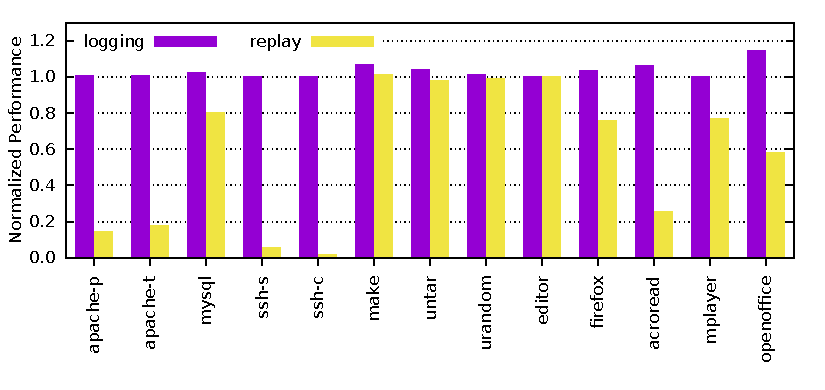
\includegraphics[width=\linewidth]{figures/scribe/overhead}
  \vspace{-5em}
  \caption{{\bf Recording Runtime Overhead.}}
  \label{scribe:fig:overhead}
\end{figure}

\begin{figure}[t]
    \centering
    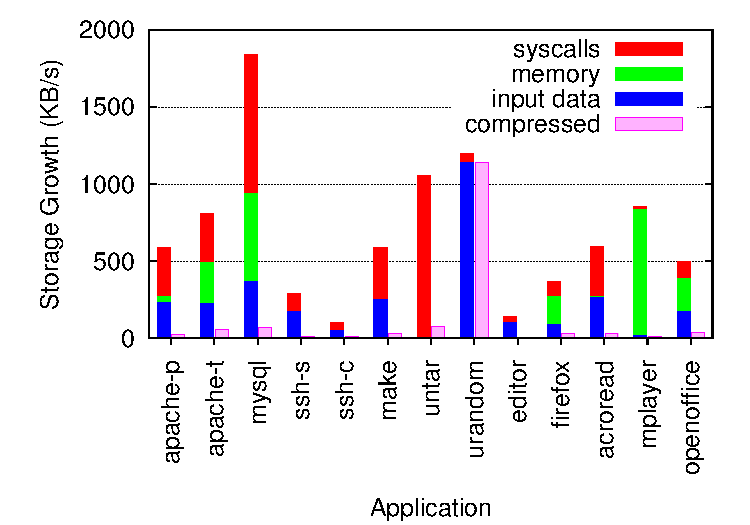
\includegraphics[width=\linewidth]{figures/scribe/storage}
  \vspace{-5em}
  \caption{{\bf Recording Storage Growth.}}
    \label{scribe:fig:storage}
\end{figure}

\begin{figure}[t]
    \centering
    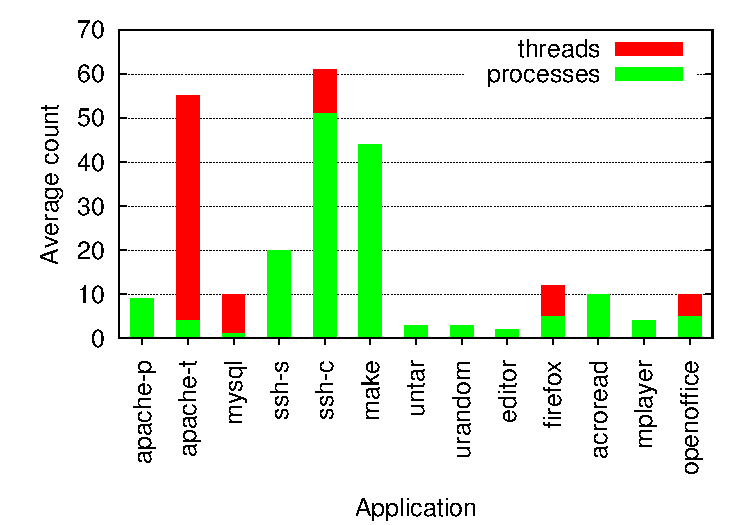
\includegraphics[width=\linewidth]{figures/scribe/totals}
  \vspace{-5em}
  \caption{{\bf Number of Processes and Threads.}}
    \label{scribe:fig:totals}
\end{figure}

\begin{figure}[t]
    \centering
    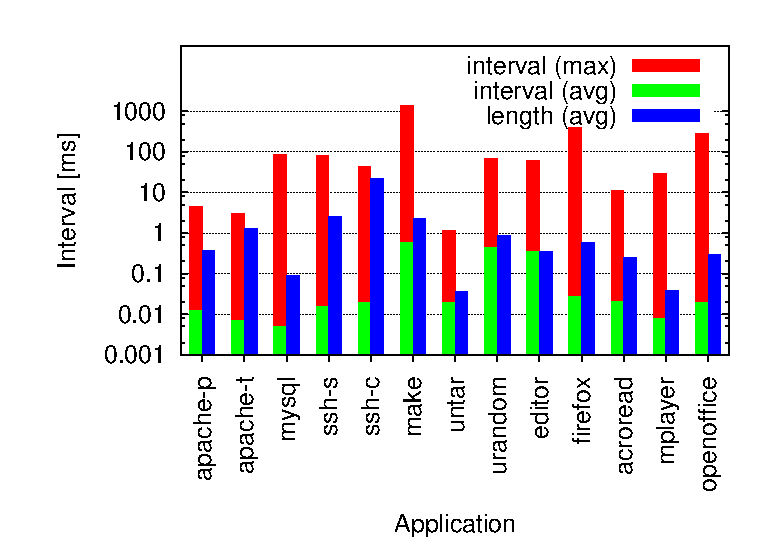
\includegraphics[width=\linewidth]{figures/scribe/syncpts2}
  \vspace{-5em}
  \caption{{\bf Sync Points Interval and Length.}}
    \label{scribe:fig:syncpts}
\end{figure}

\begin{figure}[t]
    \centering
    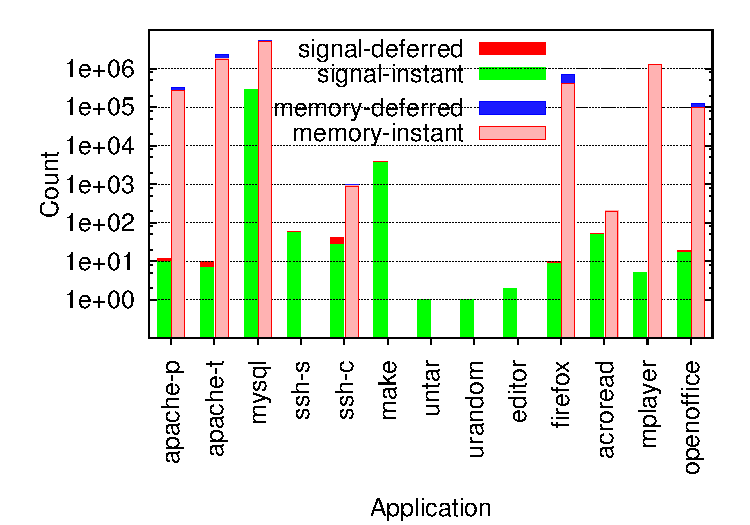
\includegraphics[width=\linewidth]{figures/scribe/stats}
  \vspace{-5em}
  \caption{{\bf Count of Signals and Memory.}}
    \label{scribe:fig:stats}
\end{figure}

\begin{figure}[t]
    \centering
    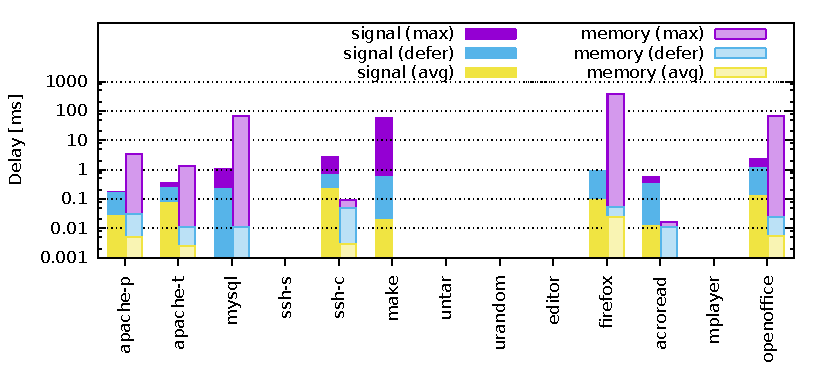
\includegraphics[width=\linewidth]{figures/scribe/delays2}
  \vspace{-5em}
  \caption{{\bf Delay of Signals and Memory.}}
    \label{scribe:fig:delays}
\end{figure}


Two factors contribute to replay speedup: omitted in-kernel work due
to system calls partially or entirely skipped (e.g. network output),
and compressed time due to time waiting skipped at replay (e.g. timer
expiration). Application that do neither perform the same work whether
recording or replaying, and sustain speedups close to 1. This includes
computation-intensive workloads such as {\tt make}, {\tt urandom},
{\tt untar}, and {\tt editor}. The speedup increases as the workload
exhibits more idle time in sleeping or blocking (mostly waiting for
input events). For instance, {\tt mplayer} spends about 23\% of the
time sleeping during recording, and its replay speedup is roughly
1.3. Replay speedup is noticeably larger for workloads
that spend much of their time sleeping: 3.9 for {\tt acrobat},
7.1 for {\tt apache-p}, and 5.8 for {\tt apache-t}.
Interactive workloads obtained
the largest speedups: 19 for {\tt ssh-s} and 70 for {\tt ssh-c}.

Figure~\ref{scribe:fig:storage} shows the storage growth rate of recording.
Storage requirements are decomposed into memory-related events ({\tt
  memory}), nondeterministic input data returned by system calls ({\tt
  input data}), and other data which is primarily system call return
values and rendezvous points ({\tt syscalls}).  The storage growth
rates ranged from 100\KB{}/\secs{} for {\tt ssh-c} to almost
1.9\MB{}/\secs{} for {\tt mysql}.  These storage requirements are
quite modest.  When compressed using lzma, storage growth rates
dropped to between 1 to 90\KB{}/\secs{} for all scenarios except {\tt
  urandom}, whose storage growth rate 
remained a bit over 1.1\MB{}/\secs{}.  Most of the log of
{\tt urandom} is due to input of random data, which does not compress
well.  

Figure~\ref{scribe:fig:totals} shows the average number of processes and
threads running for each application scenario.  The sum of the two is
the average number of total Linux tasks running.  All workloads except {\tt
  editor} consisted of multiple processes or threads, demonstrating
\scribe{}'s ability to record and replay real multi-process and
multi-threaded application workloads.  Five of the scenarios used
threads: {\tt apache-t}, {\tt mysql}, {\tt ssh-c}, {\tt firefox}, and 
{\tt openoffice}. For all of these scenarios except {\tt ssh-c}, this
correlates with the majority of the log storage consisting of memory
events, as shown in Figure~\ref{scribe:fig:storage}.  The threads in {\tt
  ssh-c} are
used in the benchmark to manage
concurrent sessions.  They involve very little contention over shared
memory, and therefore do not contribute much to the log size.
Conversely, {\tt apache-p} shows mild shared memory activity despite
being a multi-process application rather than multi-threaded. 

Figure~\ref{scribe:fig:syncpts} shows the time interval between consecutive
per process sync points for each application scenario. The average
time interval is measured per process then averaged over all
processes.  It is at most 30\us{} for all scenarios except {\tt make},
{\tt urandom} and {\tt editor}, for which it is less than 500\us{}.
These three are CPU intensive workloads that produce sync points only
due to system calls.
The maximum time interval between sync points for almost all
application workloads was less than 100\ms{}, which is also not large
and similar to the scheduling time quantum in Linux.  The maximum time
interval for three application workloads, {\tt make}, {\tt firefox},
and {\tt openoffice}, was higher, but only occurred once,
during the startup of each application.  If we exclude these outliers
and compute the 99th percentile of the time interval between sync
points, the time interval is less than 10\ms{}.

Figure~\ref{scribe:fig:syncpts} also shows the average length of sync points
per process for each application scenario. It is at least 300\us{} for
all scenarios except {\tt untar} and {\tt mplayer}, in which it is
over 50\us{}. More importantly, in all workloads the average time
spent at a sync point is significantly larger---over an order of
magnitude in most cases---than the time spent between sync point, or
outside sync points. Processes persist longer at sync points whenever,
for example, they block on I/O in a system call or wait for page
ownership transfer. During the time intervals within sync points,
asynchronous events for a process are delivered instantly and need not
be deferred. In other words, on average, most of the time asynchronous
events can be delivered promptly; and if not, then they are delayed
for a short period.  This establishes the empirical grounds for
\scribe{}'s reliance on sync points to successfully convert
asynchronous events to synchronous ones in a timely manner.

Figure~\ref{scribe:fig:stats} shows the total number of signals and shared
memory page faults due to \scribe{}'s page ownership management mechanism
for each application scenario.  Page faults not due to \scribe{} are
not included.  The totals are decomposed into those that are handled
instantly versus those that need to be deferred until a sync point is
reached.  The measurements show that \scribe{} provides
low-overhead execution recording even in the presence of a large
number of asynchronous events.  
Nearly all asynchronous events of
either type are handled instantly as they arrive, because the process
that is the target of these events is already executing in the
kernel at a sync point.  Sync points not only happen frequently
enough, but also endure long enough, that the vast majority of
asynchronous events can be handled immediately without being deferred.

Observe in Figure~\ref{scribe:fig:stats} that asynchronous events due to
shared memory page faults predominate over signals in scenarios that
involve multiple threads or shared memory. In these scenarios, page
faults due to \scribe{}'s page ownership management occur in larger
numbers, and, since they themselves are sync points, they contribute
to the pool of available sync points. The fraction of sync points due
to shared memory page faults of the total number of sync points ranges
from 10\% in {\tt apache-p}, to 30\% in {\tt mysql}, {\tt apache-t},
{\tt firefox}, and {\tt openoffice}, and up to 50\% in {\tt mplayer}.
In other words, applications that need sync points for shared memory
accesses are also likely to have sync points more frequently.

Figure~\ref{scribe:fig:delays} shows the amount of delay incurred for signals
and shared memory accesses. Signals were delayed at most 100\us{}
on average, except {\tt ssh-c}, which reached 220\us{}. The average
delay for only those few deferred signals that could not be handled
instantly was at most 1\ms{}. CPU intensive workloads without shared
memory produce sync points only due to system calls, and sustain longer
delays for deferred signals.  For example, in {\tt make}, 135 {\tt SIGCHLD}
signals were deferred as the parent process waited to be scheduled
while compilations occupied the CPUs. Only when it was scheduled, it
reached a sync point and handled the signal. However, even without
\scribe{}, when the signal is delivered instantly, the parent process
would only handle the signal after a comparable delay since it would
still wait to be scheduled.  In multi-threaded workloads, the
delays for signals are longer, despite the addition of sync points due
to shared memory accesses. This is because our prototype only
considered sync points due to system calls for deferred signals. The
delays would probably be more comparable to those for shared memory
access if sync points due to shared memory were also used.

Unlike with signals, when a shared memory event occurs, the process
that faulted blocks until access is granted. Thus, whether memory
events are delayed and for how long is pivotal for the performance of
the system. Fortunately, shared memory accesses introduce numerous
additional sync points due to page ownership transfers. The average
delay for shared memory accesses was less than 25\us{}. If we consider
only deferred shared memory accesses that could not be handled
instantly, the average delay increases modestly to at most 60\us{}.
These delays are comparable to the native service time of a page
fault. \scribe{}'s sync points convert page ownership transfers from
asynchronous events to synchronous events with negligible impact on
page fault performance, since most asynchronous events are handled
instantaneously.

Finally, through all the executions of the application scenarios,
we have never observed a situation in which a process failed to reach a sync
point in a reasonable time, or at all.  Although \scribe{} has a 
mechanism in place to deal with delays that become too large, we did
not witness a need for this functionality in practice.  
Our experiences and results demonstrate that sync points occur
frequently and are useful for enabling deterministic replay.

\section{Related Work}
\label{scribe:sec:related}

Replaying program execution has been of interest for over 40
years~\cite{exdams}.  Hardware
mechanisms~\cite{hwrr,dmp,rerun,delorean,capo,strata,bugnet,fdr}
face a high implementation barrier and do not support record-replay on
commodity hardware.  Virtual machine
mechanisms~\cite{bressoud,revirt,smp-revirt,vmware}
require replaying operating system execution just to replay
application execution.  Almost none of them support replaying
multiprocessor virtual machines, and the ones that do incur an order
of magnitude worse overhead for common applications like
compilation due to kernel-level sharing, such as writing files to the
same directory~\cite{smp-revirt}. Most of application and 
library mechanisms~\cite{liblog,r2:osdi,kendo,jockey} cannot provide
transparent record-replay for unmodified applications.
Only one practical userspace solution exists, Mozilla~rr~\cite{mozilla-rr}.
While it provides a comprehensive set of features, it does not support
multiprocessor record-replay.  Programming
language mechanisms~\cite{dejavu,instant-replay,replay-pldi} do not
support widely-used applications written in languages that do not
provide record-replay primitives.  Unlike these approaches, \scribe{}
is an operating system mechanism.  It works at a higher-level
abstraction than hardware or virtual machine approaches to reduce
recording overhead.  It works at a lower-level abstraction than
application, library, and programming language approaches to provide
transparent record-replay for unmodified applications.

Other operating system mechanisms have also been
proposed~\cite{rr,bressoud-tft,srinivasan:flashback,rr-realtime} that interpose
between applications and the operating system.  None of them
provides record-replay for multi-threaded and
multi-process applications.  In fact, only TFT~\cite{bressoud-tft}
shows any record-replay results for real applications, namely 
{\tt gzip}, a single process application, but overhead was
quite high.  Unlike \scribe{}, TFT is only designed to replay a single
process.  Debugging using deterministic replay (DUDR)~\cite{rr-realtime}
presents only a paper design with no implementation or evaluation,
while Flashback~\cite{srinivasan:flashback} and RR~\cite{rr} are largely
incomplete with no results beyond those for a single, simple test
program.  In contrast, \scribe{} demonstrates for the first time that
record-replay of real multi-threaded and multi-process applications is
possible using an operating system approach.  

A key issue for operating system mechanisms is replaying the in-kernel
side effects of system calls.  This must be done for at least some
system calls in all replay systems.  
Previous approaches
do not solve the important problem of nondeterminism arising from
the order of execution of related system calls.  TFT only replays a
single process, so this issue does not arise.  DUDR and Flashback
hypothesize counting instructions to know when context switches occur
to track exact scheduling order to know the order of system call
execution among processes.  However, they provide no mechanism for
obtaining and using the required cycle accurate counters, and the
approach itself does not work for multiprocessors.  RR suggests
instrumenting the system call interface, but provides no actual
mechanism to do it.  In contrast, \scribe{} provides a new mechanism
using rendezvous points that solves this problem without tracking
exact scheduling order.  \scribe{}'s mechanism does not require
hardware support and works for multiprocessor systems. 

Record-replay systems must record the exact location in an instruction
stream at which an asynchronous event occurs.
This can be done by adding hardware support, modifying
applications, or writing applications with new language primitives to
record exactly when the application receives the event.
To do this on commodity hardware without application changes, all
previous approaches that deal with this
issue~\cite{bressoud,revirt,smp-revirt,slye96}
rely on the existence of a cycle accurate instruction counter.
To deal with interrupt lag~\cite{hwcount-isas06}, replay is done by
interrupting execution some time before the asynchronous event should
occur, 
setting a breakpoint on the instruction at which it should
occur, then stopping at every breakpoint to see if the instruction
counter matches the recorded value.  When they match, the asynchronous
event is delivered.
In contrast, \scribe{} introduces a fundamentally
different mechanism based on sync points that does not rely on
hardware performance counters.

TFT~\cite{bressoud-tft} proposed recording in periodic epochs for
fault tolerance, and then deferring the delivery of signals 
sent in each epoch until the respective epoch ends.  Epochs are
created by instrumenting applications to use counters to periodically
return control to TFT.  This also makes it easier to determine when
signals are delivered since they are delivered at well-defined epoch
boundaries.  The idea is similar to \scribe{}'s notion of deferring
signal delivery until sync points.  But, unlike TFT, \scribe{}
does not require instrumenting applications and does not define sync
points based on any measure of time or instruction counts.  Instead,
sync points are based on system calls, page faults, and traps that
occur as part of normal application execution.  Unlike TFT which only
supports replaying a single process, \scribe{} uses sync points to
enable replay of multi-process and multi-threaded applications on
multiprocessors. 

Besides \scribe{}, only SMP-ReVirt~\cite{smp-revirt} can transparently
replay multiprocessor workloads that use shared memory.
SMP-ReVirt replays multiprocessor virtual machines where multiple CPUs
may access shared memory.  It uses standard page protection to detect
memory races, and the concurrent read, exclusive write (CREW)
protocol~\cite{crew,instant-replay}.  To record exactly when page
access permissions switch from one CPU to another, SMP-ReVirt records
counter values in the same manner as it does for handling other
asynchronous events.  RR~\cite{rr} proposes a mechanism similar to
SMP-ReVirt, but notes problems with inaccuracy of hardware counters on
modern CPUs and has no record-replay results for any applications.
In contrast, \scribe{} avoids counter inaccuracies and introduces sync
points based on the 
assumption that real
applications perform frequent system activities that involve the
kernel.  This assumption is the antithesis of SMP-ReVirt's virtual
machine approach which must also record kernel execution.
For example, SMP-ReVirt incurs an order of magnitude worse
overhead than \scribe{} for kernel compilation due to frequent system
activities that result in kernel-level sharing.  While SMP-ReVirt can
provide whole system replay, \scribe{} can provide much more efficient
application replay.   

\section{Summary}
\label{scribe:sec:conclusion}

\scribe is the first operating system mechanism to provide transparent,
deterministic execution record and replay of multi-threaded and multi-process
applications on commodity multiprocessors and operating systems. \scribe records
and replays multiple processes by accounting for nondeterministic interactions
among processes and their execution environment.  \scribe introduces {\em
rendezvous points} to ensure correct partial ordering of execution based on
system call dependencies, and {\em sync points} to convert asynchronous
interactions that can occur at arbitrary times into synchronous events that are
much easier to record and replay.
Using these two mechanisms, \scribe overcomes the need of enforcing the original
application scheduling. While a replayed execution is different from the original
one from a kernel perspective, they appear identical from an application
perspective. By relaxing the amount of determinism
replicated at the kernel level, \scribe{} recording overhead stays modest for
various server and desktop applications without sacrificing faithfulness at the
application level.
\scribe can transition an application to running live at any time,
an instrumental for certain record-replay applications such as fault-tolerance,
or any form of debugging that requires the replayed instance to go live.
We built \racepro, a process race detection system based on the \scribe engine,
that leverage this go-live feature when performing race triage. We describe
\racepro in the next chapter and show how it generates new executions based on
previously recorded executions.
